\chapter{Búsqueda exhaustiva}

\key{Búsqueda exhaustiva}
es un método general que se puede utilizar
para resolver casi cualquier problema algorítmico.
La idea es generar todas las posibles
soluciones al problema mediante fuerza bruta,
y luego seleccionar la mejor solución o contar el
número de soluciones, dependiendo del problema.

La búsqueda exhaustiva es una buena técnica
si hay suficiente tiempo para revisar todas las soluciones,
ya que la búsqueda suele ser fácil de implementar
y siempre proporciona la respuesta correcta.
Si la búsqueda exhaustiva es demasiado lenta,
pueden ser necesarias otras técnicas, como algoritmos voraces o
programación dinámica.

\section{Generando subconjuntos}

\index{subconjunto}

Primero consideramos el problema de generar
todos los subconjuntos de un conjunto de $n$ elementos.
Por ejemplo, los subconjuntos de $\{0,1,2\}$ son
$\emptyset$, $\{0\}$, $\{1\}$, $\{2\}$, $\{0,1\}$,
$\{0,2\}$, $\{1,2\}$ y $\{0,1,2\}$.
Hay dos métodos comunes para generar subconjuntos:
podemos realizar una búsqueda recursiva
o aprovechar la representación en bits de los enteros.

\subsubsection{Método 1}

Una forma elegante de recorrer todos los subconjuntos
de un conjunto es utilizar recursión.
La siguiente función \texttt{busqueda}
genera los subconjuntos del conjunto
$\{0,1,\ldots,n-1\}$.
La función mantiene un vector \texttt{subconjunto}
que contendrá los elementos de cada subconjunto.
La búsqueda comienza cuando se llama
a la función con el parámetro 0.

\begin{lstlisting}
void busqueda(int k) {
    if (k == n) {
        // procesar subconjunto
    } else {
        busqueda(k+1);
        subconjunto.push_back(k);
        busqueda(k+1);
        subconjunto.pop_back();
    }
}
\end{lstlisting}

Cuando se llama a la función \texttt{busqueda}
con el parámetro $k$,
decide si incluir o no el
elemento $k$ en el subconjunto,
y en ambos casos,
luego se llama a sí misma con el parámetro $k+1$.
Sin embargo, si $k=n$, la función se da cuenta de que
todos los elementos han sido procesados
y se ha generado un subconjunto.

El siguiente árbol ilustra las llamadas a funciones cuando $n=3$.
Siempre podemos elegir la rama izquierda
($k$ no está incluido en el subconjunto) o la rama derecha
($k$ está incluido en el subconjunto).

\begin{center}
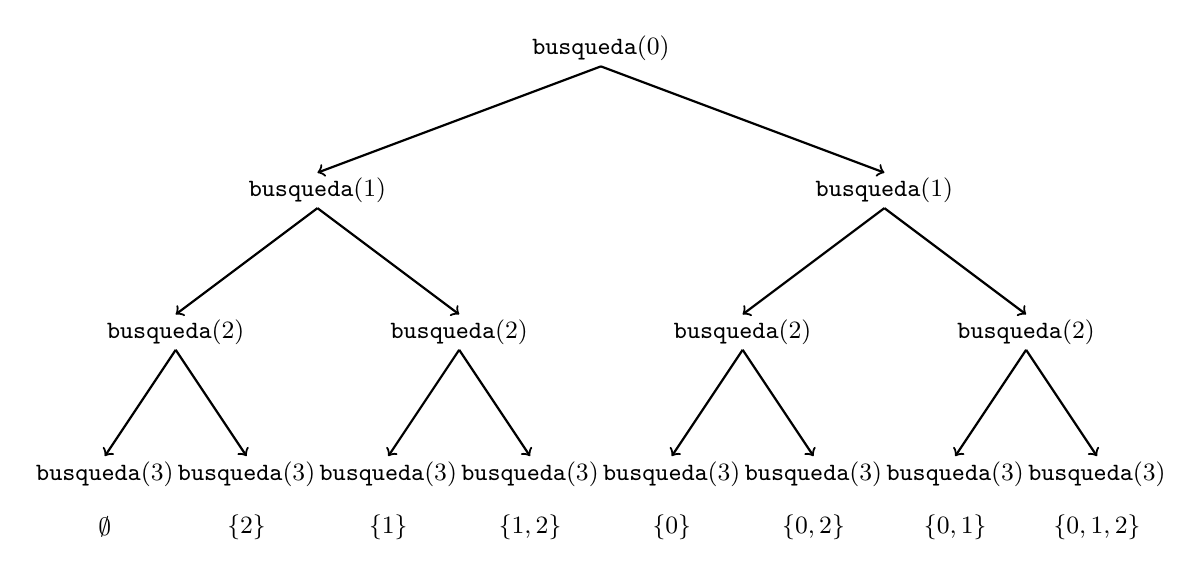
\begin{tikzpicture}[scale=.45]
  \begin{scope}
    \small
    \node at (0,0) {$\texttt{busqueda}(0)$};

    \node at (-8,-4) {$\texttt{busqueda}(1)$};
    \node at (8,-4) {$\texttt{busqueda}(1)$};

    \path[draw,thick,->] (0,0-0.5) -- (-8,-4+0.5);
    \path[draw,thick,->] (0,0-0.5) -- (8,-4+0.5);

    \node at (-12,-8) {$\texttt{busqueda}(2)$};
    \node at (-4,-8) {$\texttt{busqueda}(2)$};
    \node at (4,-8) {$\texttt{busqueda}(2)$};
    \node at (12,-8) {$\texttt{busqueda}(2)$};

    \path[draw,thick,->] (-8,-4-0.5) -- (-12,-8+0.5);
    \path[draw,thick,->] (-8,-4-0.5) -- (-4,-8+0.5);
    \path[draw,thick,->] (8,-4-0.5) -- (4,-8+0.5);
    \path[draw,thick,->] (8,-4-0.5) -- (12,-8+0.5);

    \node at (-14,-12) {$\texttt{busqueda}(3)$};
    \node at (-10,-12) {$\texttt{busqueda}(3)$};
    \node at (-6,-12) {$\texttt{busqueda}(3)$};
    \node at (-2,-12) {$\texttt{busqueda}(3)$};
    \node at (2,-12) {$\texttt{busqueda}(3)$};
    \node at (6,-12) {$\texttt{busqueda}(3)$};
    \node at (10,-12) {$\texttt{busqueda}(3)$};
    \node at (14,-12) {$\texttt{busqueda}(3)$};

    \node at (-14,-13.5) {$\emptyset$};
    \node at (-10,-13.5) {$\{2\}$};
    \node at (-6,-13.5) {$\{1\}$};
    \node at (-2,-13.5) {$\{1,2\}$};
    \node at (2,-13.5) {$\{0\}$};
    \node at (6,-13.5) {$\{0,2\}$};
    \node at (10,-13.5) {$\{0,1\}$};
    \node at (14,-13.5) {$\{0,1,2\}$};


    \path[draw,thick,->] (-12,-8-0.5) -- (-14,-12+0.5);
    \path[draw,thick,->] (-12,-8-0.5) -- (-10,-12+0.5);
    \path[draw,thick,->] (-4,-8-0.5) -- (-6,-12+0.5);
    \path[draw,thick,->] (-4,-8-0.5) -- (-2,-12+0.5);
    \path[draw,thick,->] (4,-8-0.5) -- (2,-12+0.5);
    \path[draw,thick,->] (4,-8-0.5) -- (6,-12+0.5);
    \path[draw,thick,->] (12,-8-0.5) -- (10,-12+0.5);
    \path[draw,thick,->] (12,-8-0.5) -- (14,-12+0.5);
\end{scope}
\end{tikzpicture}
\end{center}

\subsubsection{Método 2}

Otra forma de generar subconjuntos se basa en
la representación de bits de los enteros.
Cada subconjunto de un conjunto de $n$ elementos
puede representarse como una secuencia de $n$ bits,
que corresponde a un entero entre $0 \ldots 2^n-1$.
Los unos en la secuencia de bits indican
qué elementos se incluyen en el subconjunto.

La convención habitual es que
el último bit corresponde al elemento 0,
el penúltimo bit corresponde al elemento 1,
y así sucesivamente.
Por ejemplo, la representación de bits de 25
es 11001, que corresponde al subconjunto $\{0,3,4\}$.

El siguiente código recorre los subconjuntos
de un conjunto de $n$ elementos

\begin{lstlisting}
for (int b = 0; b < (1<<n); b++) {
    // procesar subconjunto
}
\end{lstlisting}

El siguiente código muestra cómo podemos encontrar
los elementos de un subconjunto que corresponde a una secuencia de bits.
Al procesar cada subconjunto,
el código construye un vector que contiene los
elementos en el subconjunto.

\begin{lstlisting}
for (int b = 0; b < (1<<n); b++) {
    vector<int> subconjunto;
    for (int i = 0; i < n; i++) {
        if (b&(1<<i)) subconjunto.push_back(i);
    }
}
\end{lstlisting}

\section{Generando permutaciones}

\index{permutación}

A continuación, consideramos el problema de generar
todas las permutaciones de un conjunto de $n$ elementos.
Por ejemplo, las permutaciones de $\{0,1,2\}$ son
$(0,1,2)$, $(0,2,1)$, $(1,0,2)$, $(1,2,0)$,
$(2,0,1)$ y $(2,1,0)$.
De nuevo, hay dos enfoques:
podemos usar recursión o recorrer las
permutaciones de forma iterativa.

\subsubsection{Método 1}

Al igual que los subconjuntos, las permutaciones se pueden generar
usando recursión.
La siguiente función \texttt{buscar} recorre
las permutaciones del conjunto $\{0,1,\ldots,n-1\}$.
La función construye un vector \texttt{permutación}
que contiene la permutación,
y la búsqueda comienza cuando se llama a la función
sin parámetros.

\begin{lstlisting}
void buscar() {
    if (permutacion.size() == n) {
        // procesar permutación
    } else {
        for (int i = 0; i < n; i++) {
            if (elegido[i]) continue;
            elegido[i] = true;
            permutacion.push_back(i);
            buscar();
            elegido[i] = false;
            permutacion.pop_back();
        }
    }
}
\end{lstlisting}

Cada llamada a la función añade un nuevo elemento a
\texttt{permutacion}.
El array \texttt{elegido} indica cuáles
elementos ya están incluidos en la permutación.
Si el tamaño de \texttt{permutacion} es igual al tamaño del conjunto,
se ha generado una permutación.

\subsubsection{Método 2}

\index{next\_permutation@\texttt{next\_permutation}}

Otro método para generar permutaciones
es comenzar con la permutación
$\{0,1,\ldots,n-1\}$ y usar repetidamente
una función que construye la siguiente permutación
en orden creciente.
La biblioteca estándar de C++ contiene la función
\texttt{next\_permutation} que se puede utilizar para esto:

\begin{lstlisting}
vector<int> permutacion;
for (int i = 0; i < n; i++) {
    permutacion.push_back(i);
}
do {
    // procesar permutacion
} while (next_permutation(permutacion.begin(),permutacion.end()));
\end{lstlisting}

\section{Backtracking}

\index{backtracking}

Un algoritmo de \key{backtracking}
comienza con una solución vacía
y extiende la solución paso a paso.
La búsqueda recursivamente
recorre todas las diferentes formas en que
se puede construir una solución.

\index{problema de las reinas}

Como ejemplo, considere el problema de
calcular el número
de formas en que $n$ reinas pueden ser colocadas en
un tablero de ajedrez $n \times n$ de tal manera que
ninguna reina ataque a las demás.
Por ejemplo, cuando $n=4$,
hay dos soluciones posibles:

\begin{center}
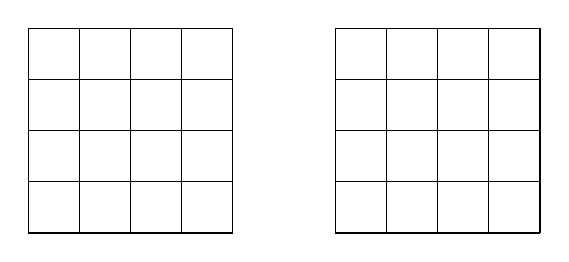
\begin{tikzpicture}[scale=.65]
  \begin{scope}
    \draw (0, 0) grid (4, 4);
    \node at (1.5,3.5) {\symqueen};
    \node at (3.5,2.5) {\symqueen};
    \node at (0.5,1.5) {\symqueen};
    \node at (2.5,0.5) {\symqueen};

    \draw (6, 0) grid (10, 4);
    \node at (6+2.5,3.5) {\symqueen};
    \node at (6+0.5,2.5) {\symqueen};
    \node at (6+3.5,1.5) {\symqueen};
    \node at (6+1.5,0.5) {\symqueen};

  \end{scope}
\end{tikzpicture}
\end{center}

El problema se puede resolver mediante backtracking
colocando reinas en el tablero fila por fila.
Más precisamente, se colocará exactamente una reina en cada fila de tal manera que ninguna reina ataque
a ninguna de las reinas colocadas anteriormente.
Se ha encontrado una solución cuando todas
las $n$ reinas han sido colocadas en el tablero.

Por ejemplo, cuando $n=4$,
algunas soluciones parciales generadas por
el algoritmo de backtracking son las siguientes:

\begin{center}
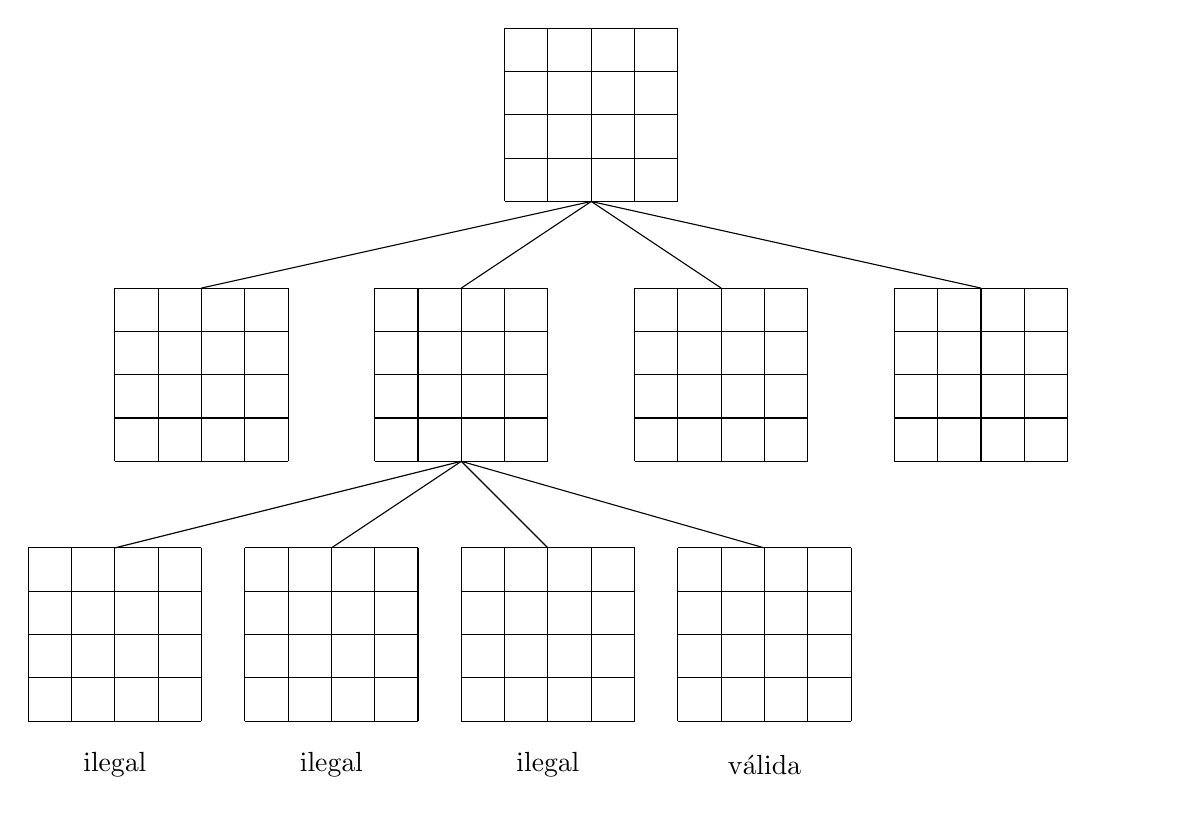
\begin{tikzpicture}[scale=.55]
  \begin{scope}
    \draw (0, 0) grid (4, 4);

    \draw (-9, -6) grid (-5, -2);
    \draw (-3, -6) grid (1, -2);
    \draw (3, -6) grid (7, -2);
    \draw (9, -6) grid (13, -2);

    \node at (-9+0.5,-3+0.5) {\symqueen};
    \node at (-3+1+0.5,-3+0.5) {\symqueen};
    \node at (3+2+0.5,-3+0.5) {\symqueen};
    \node at (9+3+0.5,-3+0.5) {\symqueen};

    \draw (2,0) -- (-7,-2);
    \draw (2,0) -- (-1,-2);
    \draw (2,0) -- (5,-2);
    \draw (2,0) -- (11,-2);

    \draw (-11, -12) grid (-7, -8);
    \draw (-6, -12) grid (-2, -8);
    \draw (-1, -12) grid (3, -8);
    \draw (4, -12) grid (8, -8);
    \draw[white] (11, -12) grid (15, -8);
    \node at (-11+1+0.5,-9+0.5) {\symqueen};
    \node at (-6+1+0.5,-9+0.5) {\symqueen};
    \node at (-1+1+0.5,-9+0.5) {\symqueen};
    \node at (4+1+0.5,-9+0.5) {\symqueen};
    \node at (-11+0+0.5,-10+0.5) {\symqueen};
    \node at (-6+1+0.5,-10+0.5) {\symqueen};
    \node at (-1+2+0.5,-10+0.5) {\symqueen};
    \node at (4+3+0.5,-10+0.5) {\symqueen};

    \draw (-1,-6) -- (-9,-8);
    \draw (-1,-6) -- (-4,-8);
    \draw (-1,-6) -- (1,-8);
    \draw (-1,-6) -- (6,-8);

    \node at (-9,-13) {ilegal};
    \node at (-4,-13) {ilegal};
    \node at (1,-13) {ilegal};
    \node at (6,-13) {válida};

  \end{scope}
\end{tikzpicture}
\end{center}

En el nivel más bajo, las tres primeras configuraciones
son ilegales, porque las reinas se atacan entre sí.
Sin embargo, la cuarta configuración es válida
y se puede extender a una solución completa colocando
dos reinas más en el tablero.
Solo hay una forma de colocar las dos reinas restantes.

\begin{samepage}
El algoritmo se puede implementar de la siguiente manera:
\begin{lstlisting}
void search(int y) {
    if (y == n) {
        count++;
        return;
    }
    for (int x = 0; x < n; x++) {
        if (column[x] || diag1[x+y] || diag2[x-y+n-1]) continue;
        column[x] = diag1[x+y] = diag2[x-y+n-1] = 1;
        search(y+1);
        column[x] = diag1[x+y] = diag2[x-y+n-1] = 0;
    }
}
\end{lstlisting}
\end{samepage}
La búsqueda comienza llamando a \texttt{search(0)}.
El tamaño del tablero es de $n \times n$,
y el código calcula el número de soluciones
en \texttt{count}.

El código asume que las filas y columnas
del tablero están numeradas de 0 a $n-1$.
Cuando se llama a la función \texttt{search} con el parámetro $y$,
coloca una reina en la fila $y$
y luego se llama a sí misma con el parámetro $y+1$.
Entonces, si $y=n$, se ha encontrado una solución
y la variable \texttt{count} se incrementa en uno.

El arreglo \texttt{column} lleva un registro de las columnas
que contienen una reina,
y los arreglos \texttt{diag1} y \texttt{diag2}
llevan un registro de las diagonales.
No está permitido agregar otra reina a una
columna o diagonal que ya contiene una reina.
Por ejemplo, las columnas y diagonales del
tablero de $4 \times 4$ están numeradas de la siguiente manera:

\begin{center}
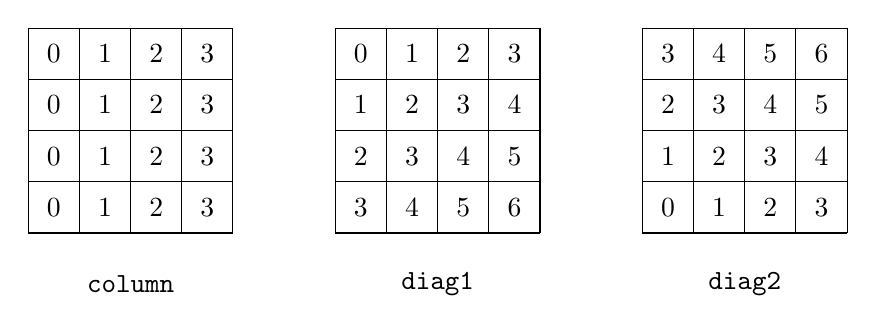
\begin{tikzpicture}[scale=.65]
  \begin{scope}
    \draw (0-6, 0) grid (4-6, 4);
    \node at (-6+0.5,3.5) {$0$};
    \node at (-6+1.5,3.5) {$1$};
    \node at (-6+2.5,3.5) {$2$};
    \node at (-6+3.5,3.5) {$3$};
    \node at (-6+0.5,2.5) {$0$};
    \node at (-6+1.5,2.5) {$1$};
    \node at (-6+2.5,2.5) {$2$};
    \node at (-6+3.5,2.5) {$3$};
    \node at (-6+0.5,1.5) {$0$};
    \node at (-6+1.5,1.5) {$1$};
    \node at (-6+2.5,1.5) {$2$};
    \node at (-6+3.5,1.5) {$3$};
    \node at (-6+0.5,0.5) {$0$};
    \node at (-6+1.5,0.5) {$1$};
    \node at (-6+2.5,0.5) {$2$};
    \node at (-6+3.5,0.5) {$3$};

    \draw (0, 0) grid (4, 4);
    \node at (0.5,3.5) {$0$};
    \node at (1.5,3.5) {$1$};
    \node at (2.5,3.5) {$2$};
    \node at (3.5,3.5) {$3$};
    \node at (0.5,2.5) {$1$};
    \node at (1.5,2.5) {$2$};
    \node at (2.5,2.5) {$3$};
    \node at (3.5,2.5) {$4$};
    \node at (0.5,1.5) {$2$};
    \node at (1.5,1.5) {$3$};
    \node at (2.5,1.5) {$4$};
    \node at (3.5,1.5) {$5$};
    \node at (0.5,0.5) {$3$};
    \node at (1.5,0.5) {$4$};
    \node at (2.5,0.5) {$5$};
    \node at (3.5,0.5) {$6$};

    \draw (6, 0) grid (10, 4);
    \node at (6.5,3.5) {$3$};
    \node at (7.5,3.5) {$4$};
    \node at (8.5,3.5) {$5$};
    \node at (9.5,3.5) {$6$};
    \node at (6.5,2.5) {$2$};
    \node at (7.5,2.5) {$3$};
    \node at (8.5,2.5) {$4$};
    \node at (9.5,2.5) {$5$};
    \node at (6.5,1.5) {$1$};
    \node at (7.5,1.5) {$2$};
    \node at (8.5,1.5) {$3$};
    \node at (9.5,1.5) {$4$};
    \node at (6.5,0.5) {$0$};
    \node at (7.5,0.5) {$1$};
    \node at (8.5,0.5) {$2$};
    \node at (9.5,0.5) {$3$};

    \node at (-4,-1) {\texttt{column}};
    \node at (2,-1) {\texttt{diag1}};
    \node at (8,-1) {\texttt{diag2}};

  \end{scope}
\end{tikzpicture}
\end{center}

Sea $q(n)$ el número de formas de
colocar $n$ reinas en un tablero de ajedrez de $n \times n$.
El algoritmo de backtracking anterior nos dice que, por ejemplo, $q(8)=92$.
Cuando $n$ aumenta, la búsqueda se vuelve rápidamente lenta,
porque el número de soluciones aumenta
exponencialmente.
Por ejemplo, calcular $q(16)=14772512$
usando el algoritmo anterior ya toma aproximadamente un minuto
en una computadora moderna\footnote{No se conoce ninguna forma eficiente de
calcular valores más grandes de $q(n)$. El récord actual es
$q(27)=234907967154122528$, calculado en 2016 \cite{q27}.}.

\section{Recorte de la búsqueda}

A menudo podemos optimizar backtracking podando el árbol de búsqueda.
La idea es agregar ''inteligencia'' al algoritmo
para que pueda notar lo más rápido posible
si una solución parcial no puede extenderse
a una solución completa.
Dichas optimizaciones pueden tener un tremendo
efecto en la eficiencia de la búsqueda.

Consideremos el problema
de calcular el número de caminos
en una cuadrícula de $n \times n$ desde la esquina superior izquierda
hasta la esquina inferior derecha, de tal manera que
el camino visite cada cuadrado exactamente una vez.
Por ejemplo, en una cuadrícula de $7 \times 7$,
hay 111712 de estos caminos.
Uno de los caminos es el siguiente:

\begin{center}
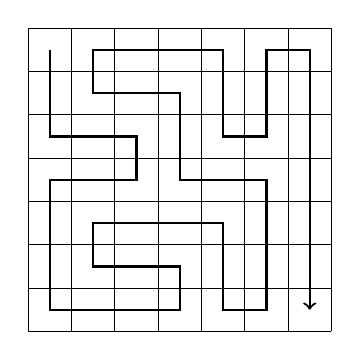
\begin{tikzpicture}[scale=.55]
  \begin{scope}
    \draw (0, 0) grid (7, 7);
    \draw[thick,->] (0.5,6.5) -- (0.5,4.5) -- (2.5,4.5) --
          (2.5,3.5) -- (0.5,3.5) -- (0.5,0.5) --
          (3.5,0.5) -- (3.5,1.5) -- (1.5,1.5) --
          (1.5,2.5) -- (4.5,2.5) -- (4.5,0.5) --
          (5.5,0.5) -- (5.5,3.5) -- (3.5,3.5) --
          (3.5,5.5) -- (1.5,5.5) -- (1.5,6.5) --
          (4.5,6.5) -- (4.5,4.5) -- (5.5,4.5) --
          (5.5,6.5) -- (6.5,6.5) -- (6.5,0.5);
  \end{scope}
\end{tikzpicture}
\end{center}

Nos enfocamos en el caso de $7 \times 7$,
porque su nivel de dificultad es apropiado para nuestras necesidades.
Comenzamos con un algoritmo de backtracking sencillo,
y luego lo optimizamos paso a paso utilizando observaciones
sobre cómo se puede podar la búsqueda.
Después de cada optimización, medimos el tiempo de ejecución
del algoritmo y el número de llamadas recursivas,
para que veamos claramente el efecto de cada
optimización en la eficiencia de la búsqueda.

\subsubsection{Algoritmo básico}

La primera versión del algoritmo no contiene
ninguna optimización. Simplemente usamos backtracking para generar
todos los caminos posibles desde la esquina superior izquierda hasta
la esquina inferior derecha y contamos el número de tales caminos.

\begin{itemize}
\item
tiempo de ejecución: 483 segundos
\item
número de llamadas recursivas: 76 mil millones
\end{itemize}

\subsubsection{Optimización 1}

En cualquier solución, primero avanzamos un paso
hacia abajo o hacia la derecha.
There are always two paths that 
are symmetric
about the diagonal of the grid
after the first step.
For example, the following paths are symmetric:

\begin{center}
\begin{tabular}{ccc}
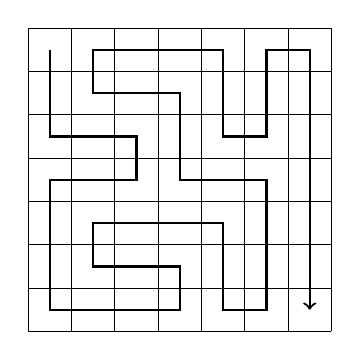
\begin{tikzpicture}[scale=.55]
  \begin{scope}
    \draw (0, 0) grid (7, 7);
    \draw[thick,->] (0.5,6.5) -- (0.5,4.5) -- (2.5,4.5) --
          (2.5,3.5) -- (0.5,3.5) -- (0.5,0.5) --
          (3.5,0.5) -- (3.5,1.5) -- (1.5,1.5) --
          (1.5,2.5) -- (4.5,2.5) -- (4.5,0.5) --
          (5.5,0.5) -- (5.5,3.5) -- (3.5,3.5) --
          (3.5,5.5) -- (1.5,5.5) -- (1.5,6.5) --
          (4.5,6.5) -- (4.5,4.5) -- (5.5,4.5) --
          (5.5,6.5) -- (6.5,6.5) -- (6.5,0.5);
  \end{scope}
\end{tikzpicture}
& \hspace{20px}
& 
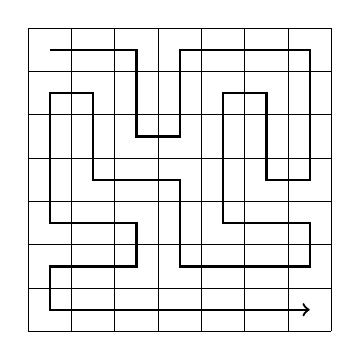
\begin{tikzpicture}[scale=.55]
  \begin{scope}[yscale=1,xscale=-1,rotate=-90]
    \draw (0, 0) grid (7, 7);
    \draw[thick,->] (0.5,6.5) -- (0.5,4.5) -- (2.5,4.5) --
          (2.5,3.5) -- (0.5,3.5) -- (0.5,0.5) --
          (3.5,0.5) -- (3.5,1.5) -- (1.5,1.5) --
          (1.5,2.5) -- (4.5,2.5) -- (4.5,0.5) --
          (5.5,0.5) -- (5.5,3.5) -- (3.5,3.5) --
          (3.5,5.5) -- (1.5,5.5) -- (1.5,6.5) --
          (4.5,6.5) -- (4.5,4.5) -- (5.5,4.5) --
          (5.5,6.5) -- (6.5,6.5) -- (6.5,0.5);
  \end{scope}
\end{tikzpicture}
\end{tabular}
\end{center}

Hence, we can decide that we always first
move one step down (or right),
and finally multiply the number of solutions by two.

\begin{itemize}
\item
running time: 244 seconds
\item
number of recursive calls: 38 billion
\end{itemize}

\subsubsection{Optimization 2}

If the path reaches the lower-right square
before it has visited all other squares of the grid,
it is clear that
it will not be possible to complete the solution.
An example of this is the following path:

\begin{center}
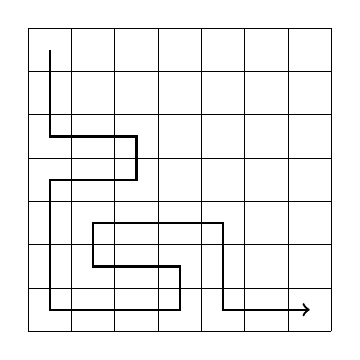
\begin{tikzpicture}[scale=.55]
  \begin{scope}
    \draw (0, 0) grid (7, 7);
    \draw[thick,->] (0.5,6.5) -- (0.5,4.5) -- (2.5,4.5) --
          (2.5,3.5) -- (0.5,3.5) -- (0.5,0.5) --
          (3.5,0.5) -- (3.5,1.5) -- (1.5,1.5) --
          (1.5,2.5) -- (4.5,2.5) -- (4.5,0.5) --
          (6.5,0.5);
  \end{scope}
\end{tikzpicture}
\end{center}
Using this observation, we can terminate the search
immediately if we reach the lower-right square too early.
\begin{itemize}
\item
running time: 119 seconds
\item
number of recursive calls: 20 billion
\end{itemize}

\subsubsection{Optimization 3}

If the path touches a wall
and can turn either left or right,
the grid splits into two parts
that contain unvisited squares.
For example, in the following situation,
the path can turn either left or right:

\begin{center}
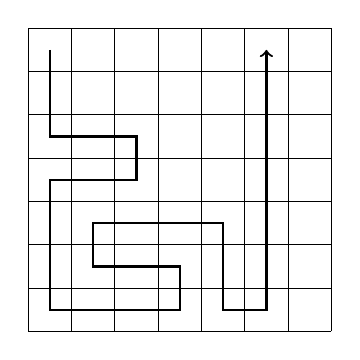
\begin{tikzpicture}[scale=.55]
  \begin{scope}
    \draw (0, 0) grid (7, 7);
    \draw[thick,->] (0.5,6.5) -- (0.5,4.5) -- (2.5,4.5) --
          (2.5,3.5) -- (0.5,3.5) -- (0.5,0.5) --
          (3.5,0.5) -- (3.5,1.5) -- (1.5,1.5) --
          (1.5,2.5) -- (4.5,2.5) -- (4.5,0.5) --
          (5.5,0.5) -- (5.5,6.5);
  \end{scope}
\end{tikzpicture}
\end{center}
In this case, we cannot visit all squares anymore,
so we can terminate the search.
This optimization is very useful:

\begin{itemize}
\item
running time: 1.8 seconds
\item
number of recursive calls: 221 million
\end{itemize}

\subsubsection{Optimization 4}

The idea of Optimization 3
can be generalized:
if the path cannot continue forward
but can turn either left or right,
the grid splits into two parts
that both contain unvisited squares.
For example, consider the following path:

\begin{center}
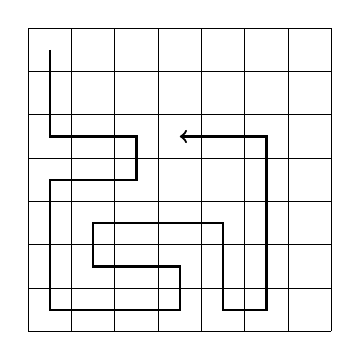
\begin{tikzpicture}[scale=.55]
  \begin{scope}
    \draw (0, 0) grid (7, 7);
    \draw[thick,->] (0.5,6.5) -- (0.5,4.5) -- (2.5,4.5) --
          (2.5,3.5) -- (0.5,3.5) -- (0.5,0.5) --
          (3.5,0.5) -- (3.5,1.5) -- (1.5,1.5) --
          (1.5,2.5) -- (4.5,2.5) -- (4.5,0.5) --
          (5.5,0.5) -- (5.5,4.5) -- (3.5,4.5);
  \end{scope}
\end{tikzpicture}
\end{center}
It is clear that we cannot visit all squares anymore,
so we can terminate the search.
After this optimization, the search is
very efficient:

\begin{itemize}
\item
running time: 0.6 seconds
\item
number of recursive calls: 69 million
\end{itemize}

~\\
Now is a good moment to stop optimizing
the algorithm and see what we have achieved.
The running time of the original algorithm
was 483 seconds,
and now after the optimizations,
the running time is only 0.6 seconds.
Thus, the algorithm became nearly 1000 times
faster after the optimizations.

This is a usual phenomenon in backtracking,
because the search tree is usually large
and even simple observations can effectively
prune the search.
Especially useful are optimizations that
occur during the first steps of the algorithm,
i.e., at the top of the search tree.

\section{Meet in the middle}

\index{meet in the middle}

\key{Meet in the middle} is a technique
where the search space is divided into
two parts of about equal size.
A separate search is performed
for both of the parts,
and finally the results of the searches are combined.

The technique can be used
if there is an efficient way to combine the
results of the searches.
In such a situation, the two searches may require less
time than one large search.
Typically, we can turn a factor of $2^n$
into a factor of $2^{n/2}$ using the meet in the
middle technique.

As an example, consider a problem where
we are given a list of $n$ numbers and
a number $x$,
and we want to find out if it is possible
to choose some numbers from the list so that
their sum is $x$.
For example, given the list $[2,4,5,9]$ and $x=15$,
we can choose the numbers $[2,4,9]$ to get $2+4+9=15$.
However, if $x=10$ for the same list,
it is not possible to form the sum.

A simple algorithm to the problem is to
go through all subsets of the elements and
check if the sum of any of the subsets is $x$.
The running time of such an algorithm is $O(2^n)$,
because there are $2^n$ subsets.
However, using the meet in the middle technique,
we can achieve a more efficient $O(2^{n/2})$ time algorithm\footnote{This
idea was introduced in 1974 by E. Horowitz and S. Sahni \cite{hor74}.}.
Note that $O(2^n)$ and $O(2^{n/2})$ are different
complexities because $2^{n/2}$ equals $\sqrt{2^n}$.

The idea is to divide the list into
two lists $A$ and $B$ such that both
lists contain about half of the numbers.
The first search generates all subsets
of $A$ and stores their sums to a list $S_A$.
Correspondingly, the second search creates
a list $S_B$ from $B$.
After this, it suffices to check if it is possible
to choose one element from $S_A$ and another
element from $S_B$ such that their sum is $x$.
This is possible exactly when there is a way to
form the sum $x$ using the numbers of the original list.

For example, suppose that the list is $[2,4,5,9]$ and $x=15$.
First, we divide the list into $A=[2,4]$ and $B=[5,9]$.
After this, we create lists
$S_A=[0,2,4,6]$ and $S_B=[0,5,9,14]$.
In this case, the sum $x=15$ is possible to form,
because $S_A$ contains the sum $6$,
$S_B$ contains the sum $9$, and $6+9=15$.
This corresponds to the solution $[2,4,9]$.

We can implement the algorithm so that
its time complexity is $O(2^{n/2})$.
First, we generate \emph{sorted} lists $S_A$ and $S_B$,
which can be done in $O(2^{n/2})$ time using a merge-like technique.
After this, since the lists are sorted,
we can check in $O(2^{n/2})$ time if
the sum $x$ can be created from $S_A$ and $S_B$.
